\section{Design of ${\Hammer}$}

Based on the observations from Section~\ref{minjia_subsec:speculation}, we introduce \Hammer, a
parallel search algorithm that exploits lightweight intra-query parallelism (i.e., path-wise parallelism and edge-wise parallelism) to accelerate the search efficiency of similarity graphs on multi-core CPU architectures. We first provide an overview of our architecture-aware design, and then we discuss technical details.

Figure~\ref{minjia_fig:fig_system_overview} depicts \Hammer's overall design that addresses the last three challenges mentioned in Section~\ref{minjia_sec:overview} to perform efficient similarity graph search.
To increase the amount of parallelism and memory bandwidth utilization (Challenge II), \Hammer uses \emph{local best-first subsearch} to deliver coarse-grained parallelism.
To limit global synchronization overhead (Challenge III), \Hammer adopts \emph{order inversion tolerance} to reduce synchronization frequency.
As such, \Hammer only requires few global synchronizations to find all near neighbors.
%(Section~\ref{minjia_subsec:loosely_sync}). 
Besides, \Hammer uses loosely synchronized visit maps for lightweight communication, adopts two-stage search to reduce unnecessary distance computations especially at the beginning, and also performs neighbor grouping technique to improve memory locality (Challenge IV). We next explain each of these techniques in detail.


%%%%%%%%%%%%
%% backup
%Figure~\ref{minjia_fig:fig_system_overview} depicts \Hammer's overall design, which is comprised of three major optimizations to address the remaining three challenges mentioned in Section~\ref{minjia_sec:overview} to perform efficient similarity graph search. To increase the amount of parallelism and memory bandwidth utilization (Challenge II), \Hammer introduces progressive multi-path expansion, which still reduces the number of convergence steps while avoiding unnecessary distance computations, especially at the beginning stage of the search (Section~\ref{minjia_subsec:progressive_MPS}). To avoid global synchronization overhead (Challenge III), \Hammer carefully handles the order inversion by lightweight synchronization on visit maps and bulk-synchronization across multiple search steps. As such, \Hammer only requires a few global synchronization to find all near neighbors (Section~\ref{minjia_subsec:loosely_sync}). To avoid irregular memory accesses (Challenge IV), \Hammer performs neighbor grouping, which flattens the similarity graph index and puts features vectors of neighbors to consecutive memory space for improved memory locality (Section~\ref{minjia_subsec:neighbor_grouping_reorder}). We next explain each of these techniques in detail.
%% end backup
%%%%%%%%%%%%


\begin{figure}[t]
    \centering
    \includegraphics[width=0.45\textwidth]{submissions/Minjia2023/figures/fig_system_overview}
    \caption{Overview of \Hammer.}
%            \emph{Dispatcher}, \emph{Executer}, and \emph{Sync Decider} are optimized in \ScaleM and \FullName.}}
    \label{minjia_fig:fig_system_overview}
\end{figure}


%%%%%%%%%%%%%%%%%%%%%%%%%%%%%%%%%%%%%%%%%%%
%%%
%\subsection{Progressive Multi-Path Search}
%\label{minjia_subsec:progressive_MPS}
%
%%%%% Introduce \ScaleM as an improvement.
%
%To investigate whether multi-path search is needed in the entire search process, we gradually increase the multi-path width (i.e., M) and the number of worker threads every $t$ steps during the search procedure. The intuition is that the search is less likely to get stuck at local minimum in the beginning of the search, so best-first search with single thread can already help the query to get close to near neighbors. As the search moves forward, it becomes more likely that a query will get stuck at local minimum and requires backtracking to escape from local minimum. Therefore, a multi-path search in later phases can better help reduce the convergence steps.  
%
%% the progressive traversal dispatcher, which gradually increases the speculation width during the search procedure to avoid the amount of redundant computations.
%
%
%% we perform 
%% % We propose \emph{progressive traversal dispatching}, which dynamically increases the width of the speculative search every $t$ steps. 
%% As shown in Section~\ref{minjia_}, the distance computations in the initial steps are often not very helpful in improving search results. This is expected, because the initial selected candidates are often random and far from the query point. Therefore, having a widened search frontier at the beginning probably would not help improve the final recall.
%% % In this case, even though speculative candidates are ranked high in visited vertices so far, they probably cannot cover the search path leading to the final nearest neighbors. Therefore, the distance computation for those speculative candidates might not be helpful for improving final recall.
%% As the search moves forward, candidates that are closer and more similar to the query would be found, and it makes more sense to increase the speculation width to cover a wider frontier for exploration. 
%
%% Taking this observation into consideration, In particular, 
%In practice, we find that a simple scaling rule works well. For example, when search begins, we first set a starting value and a maximum value for $M$. The starting value is usually one, and the maximum value can be as large as the number of available hardware threads. Subsequently, every $t$ steps (e.g., $t=1$) we double the value of $M$ until $M$ reaches its maximum. We call this dynamic increase of multi-path search width \ScaleM (\ScaleMShortName). 
%Figure~\ref{minjia_subfig:insight_1T_compt_Scale_M_vs_Top_M_vs_SGS} shows that \ScaleMShortName reduces the amount of redundant significantly in comparison to \Hammer and leads to distance computations close to \SeqShortName. On the other hand, \ScaleMShortName is able to converge as almost fast as \Hammer, as shown in 
%Figure~\ref{minjia_subfig:insight_unchecked_vs_iter_Top_M_Scale_M}. As a result, \ScaleMShortName preserves the fast convergence speeds brought by \Hammer, while with a similar amount of distance computations as \SeqShortName. 
%
%% \zhenfix{Accordingly, the number of workers will be set as equal to $M$.}
%% This way, the speculative width is constrained in the initial search steps and will be generally relaxed to the full extent.
%% The modification of doubling is called \emph{Scaling} which is an analogue to spreading phenomena in the nature.
%
%% The benefit of \ScaleMShortName is that it reduces the amount of redundant computations in the beginning of cooperative parallel search while still preserving the fast convergence properties brought by \Hammer. 
%
%%%%%% Expalin \ScaleM's advantage: 1) has almost the same convergence steps as short as Top-M reduce computation, shown in Figure~\ref{minjia_fig:insight_unchecked_vs_iter_Top_M_Scale_M}, 2) reduce distance computation, shown in Figure~\ref{minjia_fig:insight_1T_compt_Scale_M_vs_Top_M_vs_SGS}.
%%\PunchStarter{Advantage of \ScaleM}
%% As preliminary results,
%
%%\minjia{@Zhen, can you add how the number of threads changes in ScaleM? 
%%    \zhenfix{Zhen: added a sentence about how to set the number of workers.}}
%
%
%
%
%
%
%%\minjia{TODO: Can we make Figure~\ref{minjia_fig:insight_unchecked_vs_iter_Top_M_Scale_M} and Figure~\ref{minjia_fig:insight_1T_compt_Scale_M_vs_Top_M_vs_SGS} subfigs of one Figure? I'm asking because they are all about how ScaleM compares with TopM, and it seems clearer if we group them as one Figure and just refer them as Fig9.a and Fig9.b.}
%
%\begin{figure}[t]
%%    \begin{minipage}[t]{0.22\textwidth}
%        \begin{subfigure}[t]{0.23\textwidth}
%        \centering
%        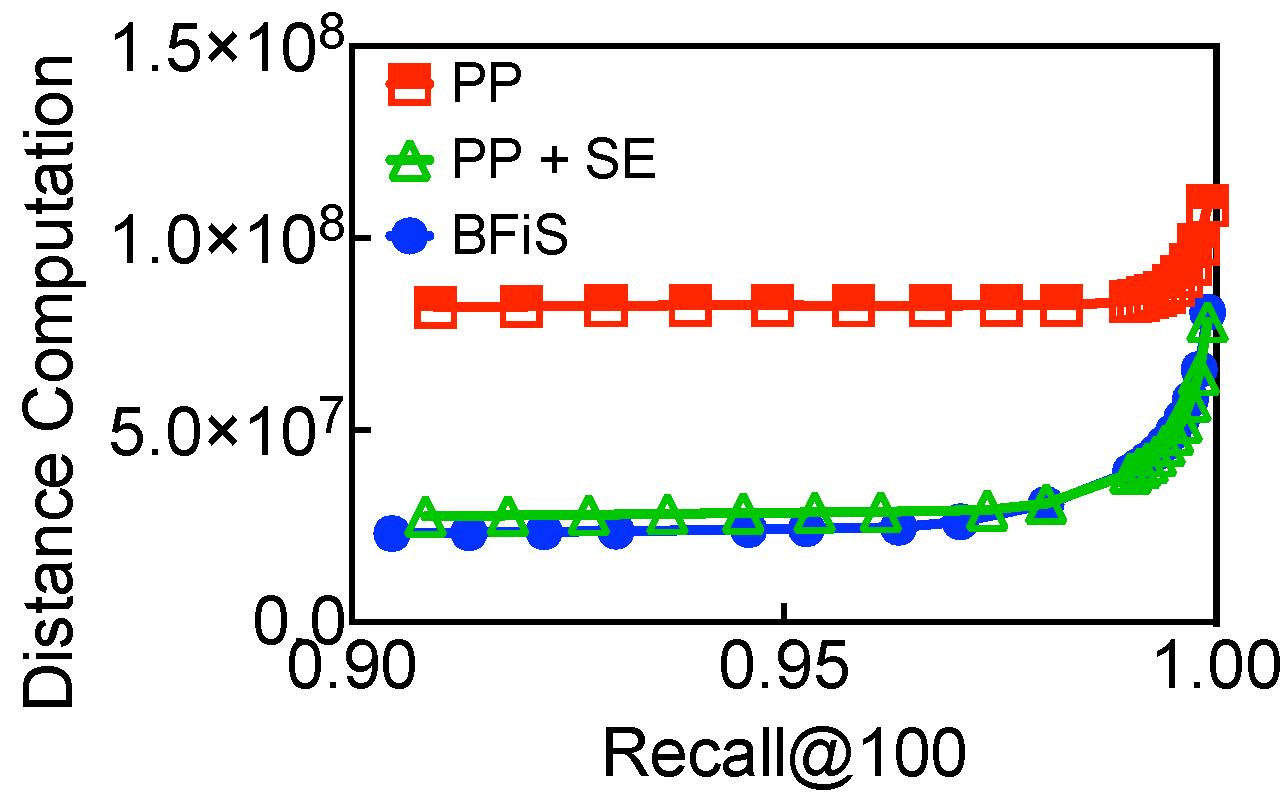
\includegraphics[height=1.1in]{submissions/Minjia2023/figures/insight_1T_compt_Scale_M_vs_Top_M_vs_SGS}
%        \caption{Distance computation of \SeqShortName, \Hammer, and \ScaleMShortName.
%                \textmd{\ScaleMShortName and \SeqShortName have similar distance computations.}}
%        \label{minjia_subfig:insight_1T_compt_Scale_M_vs_Top_M_vs_SGS}
%%    \end{minipage}
%    \end{subfigure}
%    \hfill
%%    \begin{minipage}[t]{0.22\textwidth}
%    \begin{subfigure}[t]{0.23\textwidth}
%        \centering
%        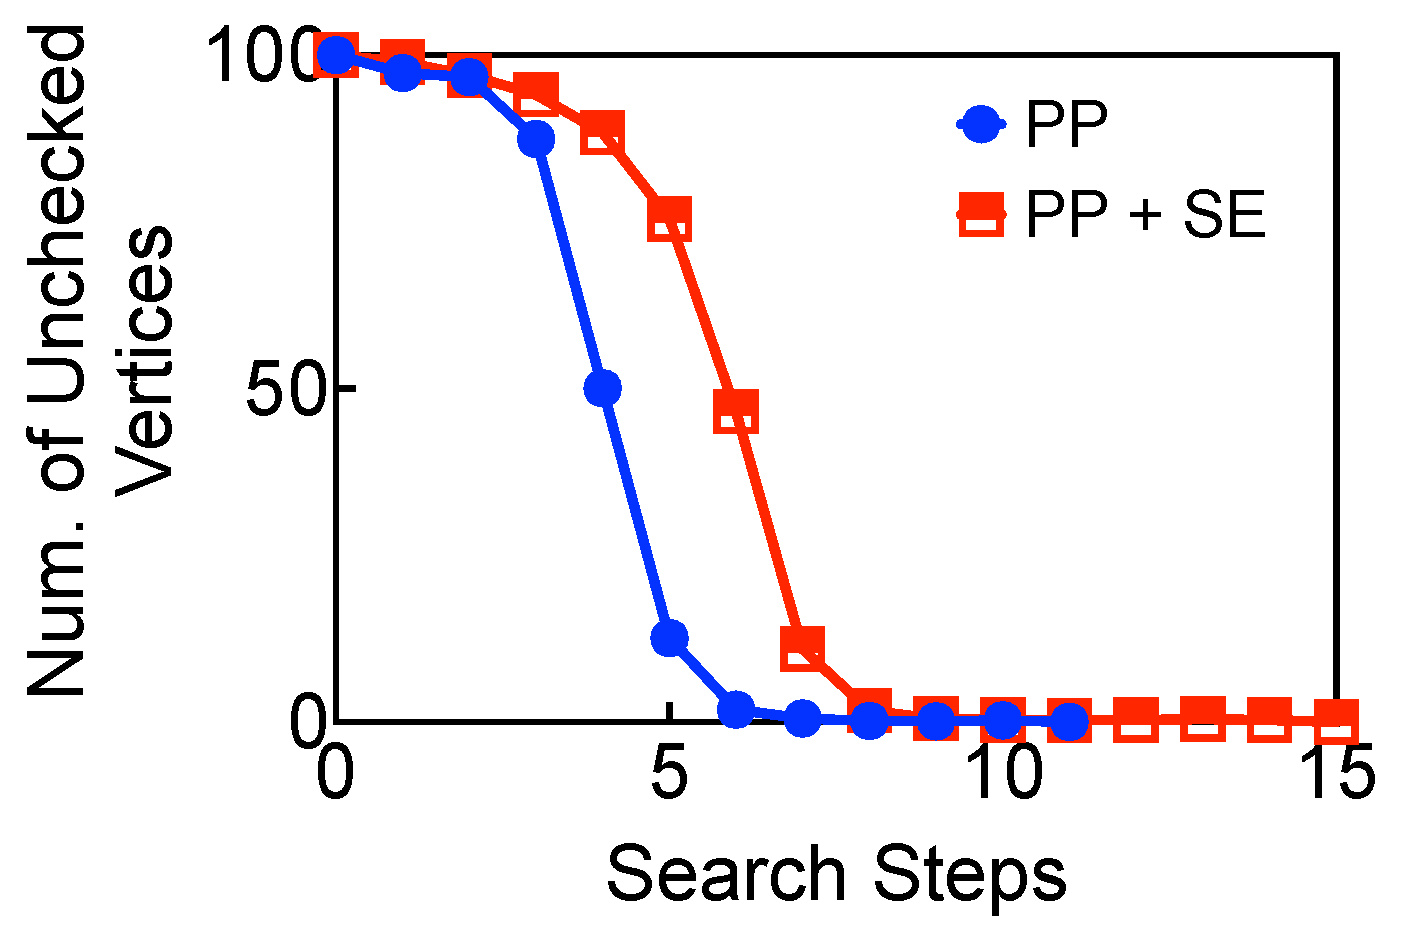
\includegraphics[height=1.05in]{submissions/Minjia2023/figures/insight_unchecked_vs_iter_Top_M_Scale_M}
%        \caption{\#unchecked candidates after each search step. 
%                \textmd{\ScaleMShortName \& \Hammer have similar numbers  of steps.}}
%        \label{minjia_subfig:insight_unchecked_vs_iter_Top_M_Scale_M}
%%    \end{minipage}
%    \end{subfigure}
%    \caption{Comparison between \Hammer and \ScaleMShortName: distance computation \& search steps.
%        \textmd{$M = 64$.}}
%    \label{minjia_fig:insight_Top_M_vs_Scale_M}
%\vspace{1em}
%\end{figure}
%%\subsubsection{\FullName Algorithm}
%%%
%%%%%%%%%%%%%%%%%%%%%%%%%%%%%%%%%%%%%%%%%%%


%\subsection{Loosely Synchronized Local-Subsearch with Bounded Order Inversion} 
\subsection{Synchronization Optimization} 
\label{minjia_subsec:loosely_sync}

%We propose \FullName (\ShortName) 
The loosely synchronized local-subsearch aims to optimize the synchronization procedure during intra-query parallel searching.
It allows multiple threads to cooperatively explore the search frontier in parallel while avoiding expensive per-step synchronization overhead. It has three important components: 
(1) a local sub-state that tracks the order from visiting a local neighborhood
and (2) delayed synchronization under certain conditions to guarantee that multiple workers still have a consistent view on the expansion order. 
Algorithm~\ref{minjia_algo:par_stale_search} depicts this part in detail. 
%(1) a local sub-state that tracks the order from visiting a local neighborhood,
%(2) loosely synchronized visit map and global candidate queue, and 
%(3) delayed synchronization under certain conditions to guarantee that multiple workers still have a consistent view on the expansion order. Algorithm~\ref{minjia_algo:par_stale_search} depicts this part in detail. 

\noindent\textbf{Local Best-First Subsearch.}
At the beginning of each global step, the global queue evenly divides its unchecked candidates among all local threads.
After that, each worker performs a local best-first search based on its own local queue of sub-states (Line~\ref{minjia_algo_line:stale_substate_start} to Line~\ref{minjia_algo_line:stale_substate_end}).
Different from the global state that involves updating the global queue, a worker's local \emph{sub-state} is the state of its own private queue.
In a local search step, a worker expands its own best unchecked candidate and updates its private queue accordingly.
Before the global queue's state is updated, a worker can have multiple sub-states of its own private queue.
%A worker continues expansion until it already has $I_{sync}$ sub-states 
A worker continues expansion until \texttt{CheckMetrics()} raises a flag for merging
or it has no unchecked candidates left locally.

In a round-robin way, a worker is assigned as the \emph{checker}. 
Her duty is to check (as what \texttt{CheckMetrics()} does) if all workers need to synchronize their sub-states by merging all private queues into the global queue.
If so (Line~\ref{minjia_algo_line:checker_true}), all workers will stop their local search and merge their queues.

The definition of \texttt{CheckMetrics()} is flexible. 
It could be a static method that no worker should do local search beyond a given step limit, or, it could be an adaptive method that uses some metrics to determine workers' dynamic status.
The details will be provided later in this section.


%The \FullName algorithm is shown in Algorithm~\ref{minjia_algo:par_stale_search}.
\begin{algorithm}[h]
\small
\DontPrintSemicolon
%\caption{\FullName (\ShortName)}\label{algo:par_stale_search}
\caption{\Hammer: Intra-Query Parallel ANNS}\label{algo:par_stale_search}
\KwIn{graph $G$, starting point $P$, query $Q$, queue capacity $L$, number of workers $T$}
\KwOut{$K$ nearest neighbors of $Q$}
expansion width $W \gets 1$\;
%global priority queue $S$ $\gets$ an empty queue with capacity $L$\;
%local priority queues $LS$ $\gets$ $T$ empty queues with capacity $L$\; \label{algo_line:stale_local_queues}
global priority queue $S$ $\gets$ an empty queue\;
local priority queues $LS$ $\gets$ $T$ empty queues\; \label{algo_line:stale_local_queues}
array $U$ $\gets$ the vector to store update positions of workers\;
compute $dist(P, Q)$ and add $P$ into $S$\;
\While{true} { \label{algo_line:stale_global_step_begin}
    divide all unchecked vertices from $S$ into $LS$\; \label{algo_line:stale_dispatching}
    % \If{all $LS$ are empty} { \label{algo_line:stale_complete_start}
    %     break\;
    %  } \label{algo_line:stale_complete_end}
    \textbf{if} all $LS$ are empty \textbf{then} break\;
    \ForEach{worker $t$ out of $W$ \textbf{in parallel}} {
        \While{$LS[t]$ has unchecked vertices {\bf and} $doMerge$ is \emph{false}} { \label{algo_line:stale_substate_start}
            $v \gets$ the first unchecked vertex in $LS[t]$\;
            mark $v$ as checked\;
            \ForEach{neighbor $u$ of $v$ in $G$} { \label{algo_line:stale_neighbor_start}
                \If{$u$ is not visited} {\label{algo_line:stale_check_map}
                    mark $u$ as visited\; \label{algo_line:stale_update_map}
                    compute $dist(u, Q)$\;
                    add $u$ into $LS[t]$\;
                }
            } \label{algo_line:stale_neighbor_end}
            \textbf{if} $LS[t]$.size() $> L$ \textbf{then} $LS[t]$.resize($L$)\;
            update $U[t]$\;
            \If{$t$ is the \emph{checker}} {
                $\bar{u} \gets$ average positions of elements in $U$\; \label{algo_line:aup_begin}
                % \If{$\bar{u} \geq L \cdot R$} { \label{algo_line:check_metric}
                %     $doMerge \gets$ \texttt{true}\; \label{algo_line:checker_true}
                % }
                % \Else {
                %     $doMerge \gets$ \texttt{false}\;
                % } \label{algo_line:aup_end}
                \textbf{if} $\bar{u} \geq L \cdot R$ \textbf{then} $doMerge \gets$ \texttt{true}\; \label{algo_line:check_metric}
                \textbf{else} $doMerge \gets$ \texttt{false}\; \label{algo_line:aup_end}
                assign the next checker in a round-robin way\;
            }
%             \If{$t$ is the \emph{checker} {\bf and} \CheckMetrics() returns \emph{true}} { \label{algo_line:checker_true}
%                 $doMerge \gets$ true\;
% %                assign the next checker in round-robin way\;
%                 assign the next checker\;
%             }
       } \label{algo_line:stale_substate_end}
    }
    merge $LS$ into $S$\; \label{algo_line:stale_merge}
    \textbf{if} $S$.size() $> L$ \textbf{then} $S$.resize($L$)\;
    \textbf{if} $W < T$ \textbf{then} $W \gets 2W$\;
} \label{algo_line:stale_global_step_end}
\Return the first $K$ vertices in $S$\;

% \Fn(\tcc*[h]{{\color{blue} by Update Position}}){\CheckMetrics()}{
% \KwIn{vector of update positions $U$, queue capacity $L$, position ratio $R$, number of workers $T$}
% \KwOut{true or false}
% $\bar{u} \gets$ average positions of elements in $U$\; \label{algo_line:aup_begin}
% \If{$\bar{u} \geq L \cdot R$} { \label{algo_line:check_metric}
%     \Return true\;
% }
% \Else {
%     \Return false\;
% } \label{algo_line:aup_end}
% }

% \minjia{@Zhen, can you actually MERGE CheckMetrics() into the main algorithm? It only has a few lines of code and feels weird to have a separate function in the pseudo code. You can do this easily by setting a flag in between line 18 and 19 and then check the flag in line 19. }


%\caption{CheckMetrics() (by Update Position)}\label{algo:check_merge_metric}
%\KwIn{vector of update positions $U$, queue capacity $L$, position ratio $R$, number of workers $T$}
%\KwOut{true or false}
%$\bar{u} \gets$ average positions of elements in $U$\;
%\If{$\bar{u} \geq L \cdot R$} { \label{algo_line:check_metric}
%    \Return true\;
%}
%\Else {
%    \Return false\;
%}
\end{algorithm}

%%%%%%%%%%%%%
%%% backup
%\begin{algorithm}
%\caption{\FullName (\ShortName)}\label{algo:par_stale_search}
%\begin{algorithmic}[1]
%\REQUIRE graph $G$, starting point $P$, query $Q$, queue capacity $L$, number of workers $T$, inner steps $I_{sync}$
%\ENSURE $K$ nearest neighbors of $Q$
%\STATE the global priority queue $S$ $\gets$ an empty queue of capacity $L$
%\STATE local priority queues $LS$ $\gets$ $T$ empty queues with capacity of $L$ \label{algo_line:stale_local_queues}
%\STATE compute $dist(P, Q)$ 
%\STATE add $P$ into $S$ 
%\WHILE{true} \label{algo_line:stale_global_step_begin}
%    \STATE divide all unchecked vertices from $S$ into $LS$ \label{algo_line:stale_dispatching}
%    \IF{all $LS$ are empty} \label{algo_line:stale_complete_start}
%        \STATE break
%    \ENDIF \label{algo_line:stale_complete_end}
%%    \STATE $ \gets 
%    \FOR{every worker $t$ \textbf{in parallel}}
%%        \STATE counter $i \gets 0$
%%        \WHILE{$i < I_{sync}$ \AND $LS[t]$ contains unchecked vertices} \label{algo_line:stale_substate_start}
%        \WHILE{$LS[t]$ contains unchecked vertices \AND $doMerge$ is \emph{false}} \label{algo_line:stale_substate_start}
%            \STATE vertex $v \gets$ the first unchecked vertex in $LS[t]$
%            \STATE mark $v$ as checked 
%            \FOR{every neighbor $u$ of $v$ in $G$} \label{algo_line:stale_neighbor_start}
%                \IF{$u$ is not visited} \label{algo_line:stale_check_map}
%                    \STATE mark $u$ as visited \label{algo_line:stale_update_map}
%                    \STATE compute $dist(u, Q)$
%                    \STATE add $u$ into $LS[t]$
%                \ENDIF
%            \ENDFOR \label{algo_line:stale_neighbor_end}
%%            \STATE $i \gets i + 1$
%            \IF{$t$ is the \emph{checker} \AND CheckMetrics() returns \emph{true}} \label{algo_line:checker_true}
%                \STATE $doMerge \gets$ true
%                \STATE assign the next checker in round-robin way
%            \ENDIF
%        \ENDWHILE \label{algo_line:stale_substate_end}
%    \ENDFOR
%    \STATE merge $LS$ into $S$ \label{algo_line:stale_merge}
%\ENDWHILE \label{algo_line:stale_global_step_end}
%\RETURN the first $K$ vertices in $S$
%\end{algorithmic}
%\end{algorithm}
%%% end backup
%%%%%%%%%%%%%



\PunchStarter{Concurrent SubTrees Expansion View.}
If we follow the earlier discussion on the tree expansion view of \SeqFullName (\SeqShortName)  and \Hammer (\Hammer), we observe the new algorithm \Hammer considering a different expansion strategy. 
Assume every unchecked vertices being initially allocated to each $LS$ (corresponding to each thread) has a virtual root node $T_r$ (Line~\ref{minjia_algo_line:stale_dispatching} in Algorithm ~\ref{minjia_algo:par_stale_search}). Then each worker grows their own subtrees rooted by $T_r$ concurrently (and independently) according to \SeqShortName.  
Only when we need to resync (Line~\ref{minjia_algo_line:stale_merge}), we produce another set of trees to expand concurrently and independently. 
Note that the trees from different threads may compete (try to visit) the same vertices, but ideally, only one thread will be able to get it. However, this may introduce significant overhead. We will introduce the loosely synchronized communication strategy to reduce such synchronization overhead in the later section. 
Note that even though $T$ threads maximally can expand $T$ tree nodes concurrently, unlike the \Hammer, such {\em parallel} expansion is asynchronous as a worker only updates its private queue until a global merging happens. 
% Note that only after $I_{sync}$ steps, they will wait to perform a global merge, which is similar to the Barrier in BSP model. 
%Importantly, the total number of synchronization in Algorithm ~\ref{minjia_algo:par_stale_search} is significantly reduced compared with \SeqShortName  and \Hammer. 
In this way, the total number of synchronization in Algorithm~\ref{minjia_algo:par_stale_search} is significantly reduced compared with \Hammer.

%%%%%%%%%%%%%%%%%%%%%%%%%%%%%%%%%%%%%%%%%%%
%%% backup
%\noindent\textbf{Loosely Synchronized Local Computation.}
%There is one potential bottleneck to multi-threaded parallel scaling in Algorithm~\ref{minjia_algo:par_stale_search} on our target architectural platforms (multi-core systems). 
%Consider visiting a neighbor of a candidate. This is typically after a check and then an update to a visiting map to ensure that a vertex is calculated once (Line~\ref{minjia_algo_line:stale_check_map}-\ref{minjia_algo_line:stale_update_map}).
%In multi-path parallel search, the visiting map is shared by all workers to indicate if a vertex has been visited.
%Since multiple threads may access the shared visiting map concurrently, locking or lock-free algorithms are required if we still want to ensure a vertex is visited only once. However, this approach involves significant scalability bottleneck, because it leads to lock contention and sequentialization of updating the visiting map.
%
%We observe that the ANN search algorithm is still correct even if a vertex is calculated multiple times, because the local candidates are guaranteed to be merged back to the global priority queue and the visiting map is also guaranteed to have \emph{eventual consistency} the next time of global synchronization. Furthermore, by inserting memory fences, cache coherence further ensures that the updated visiting map is visible to other cores. Due to the potential out-of-order execution in processors, modern multi-core processors provide \emph{fence} instructions as mechanism to override their default memory access orders. In particular, we issue a fence after a thread updates the visiting map to guarantee a processor has completed the distance computation of the corresponding vertex and has updated the visiting map (otherwise, there is no guarantee the updated visiting map is visible to other cores before next step of global synchronization).
%
%By doing the loosely synchronized local search, we observe that the search algorithm only performs a very small percentage of additional distance computations (less than 5\%) for {SIFT1M} (and similar for other datasets) with 8-way parallelism. This reduces  the overhead from synchronization by 10\% and allows us to avert the issue of non-scaling locking across multi-threading search. This optimization was also considered by Leiserson and Schardl~\cite{benign-race} (termed as "benign races") for their parallel breadth-first search algorithm. 
%Furthermore, we use a bitvector to implement the visiting map instead of a byte-array.
%% where byte is the minimum data type with Compare-and-Swap (CAS) support. 
%This optimization allows the cache to hold the largest possible portion of the visiting map and therefore improves the data locality for memory accesses. 
%%% end backup
%%%%%%%%%%%%%%%%%%%%%%%%%%%%%%%%%%%%%%%%%%%


%\noindent\textbf{Bulk-Step Synchronization with Bounded Order Inversion.} 
\noindent\textbf{Order Inversion Tolerant Search.} 
To unleash the full power of multi-core systems, \Hammer performs a unique form of \emph{order inversion tolerant} search so that worker threads do not need to synchronize at every search step in most cases. 
Specially, \emph{order inversion tolerant} means instead of having a strict order through the entire convergence steps, we allow some relaxation of the order as long as the global order becomes consistent again after a global synchronization.
% given number of steps. 
This is especially helpful for the multi-path parallel search's performance because global synchronization across multiple threads is still expensive and not very scalable as the number of cores increases. 

Figure~\ref{minjia_fig:insight_PSS_sync_frequency_vs_overhead} shows how the global synchronization frequency influences the synchronization overhead (calculated by synchronization time divided by  overall execution time) and the overall distance computations. All results in this figure return the same recall value. 
It shows that the synchronization overhead increases significantly when the synchronization frequency grows.
We also find that order inversion (without enough synchronization) slows down the search convergence and results in growing distance computations (as shown in Figure~\ref{minjia_fig:insight_PSS_sync_frequency_vs_overhead}). This is because without enough synchronization, worker threads keep searching its own (unpromising) areas without benefiting from other threads' latest search results that may lead to faster convergence. This study demonstrates that a proper synchronization frequency is desired to achieve high system performance.  


\begin{figure}[t]
    \begin{minipage}[t]{0.23\textwidth}
        \centering
        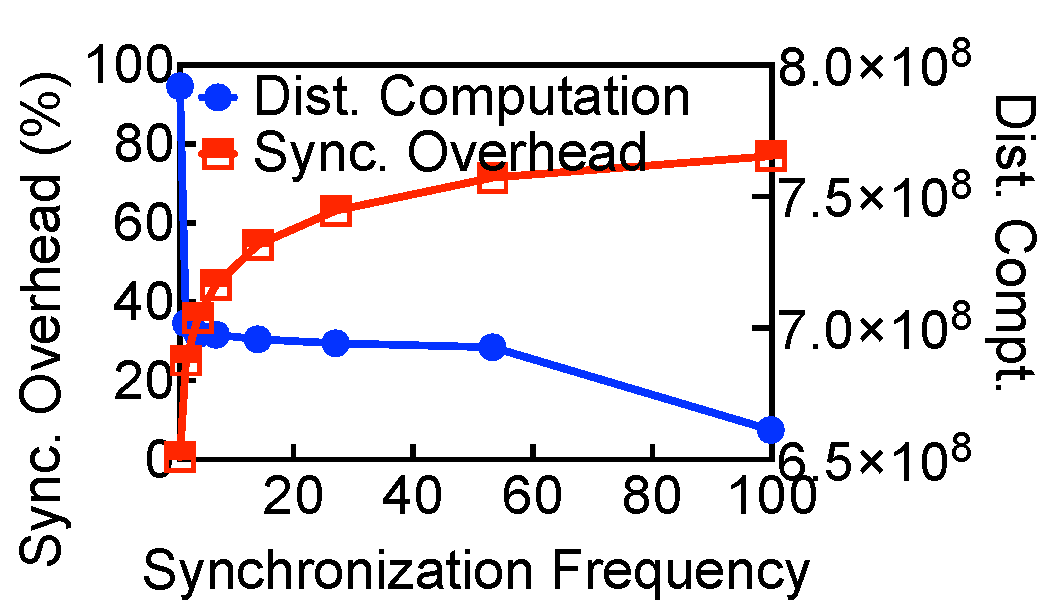
\includegraphics[height=0.98in]{submissions/Minjia2023/figures/insight_PSS_sync_frequency_vs_overhead}
        \caption{\Hammer's sync. overhead and distance computation vs. sync. frequency.}
        \label{minjia_fig:insight_PSS_sync_frequency_vs_overhead}
    \end{minipage}
    \hfill
    \begin{minipage}[t]{0.23\textwidth}
        %        \centering
        %        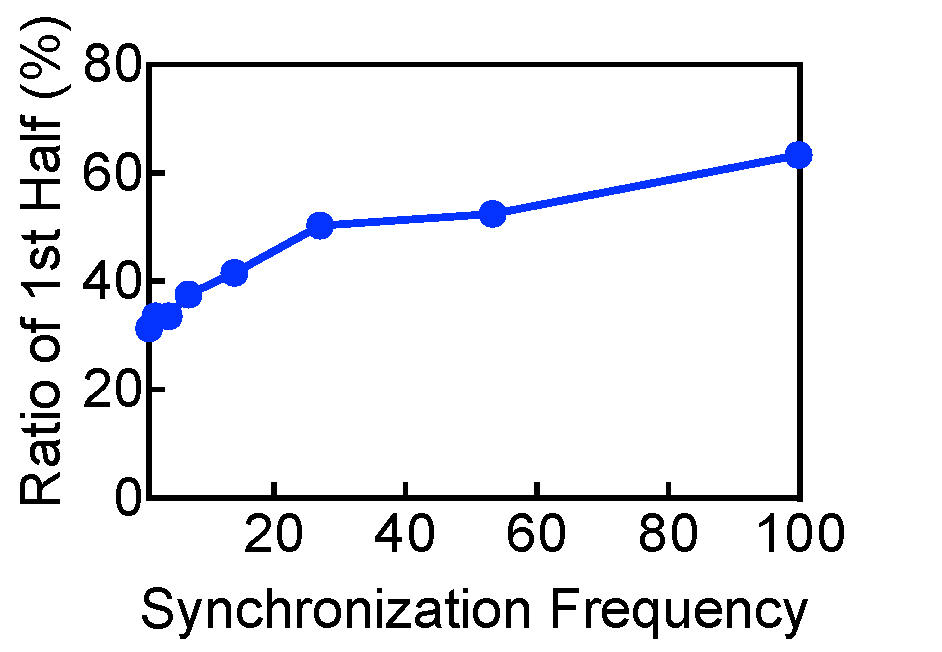
\includegraphics[height=0.98in]{submissions/Minjia2023/figures/insight_PSS_sync_frequency_vs_ratio_1st_half}
        %        \caption{Ratio of the average update position in the 1st half of private queues.
            %            %\textmd{When $M$ is increasing, \Hammer's search steps are declining while its distance computation is increasing.}
            %        }
        %        \label{minjia_fig:insight_PSS_sync_frequency_vs_ratio_1st_half}
        \centering
        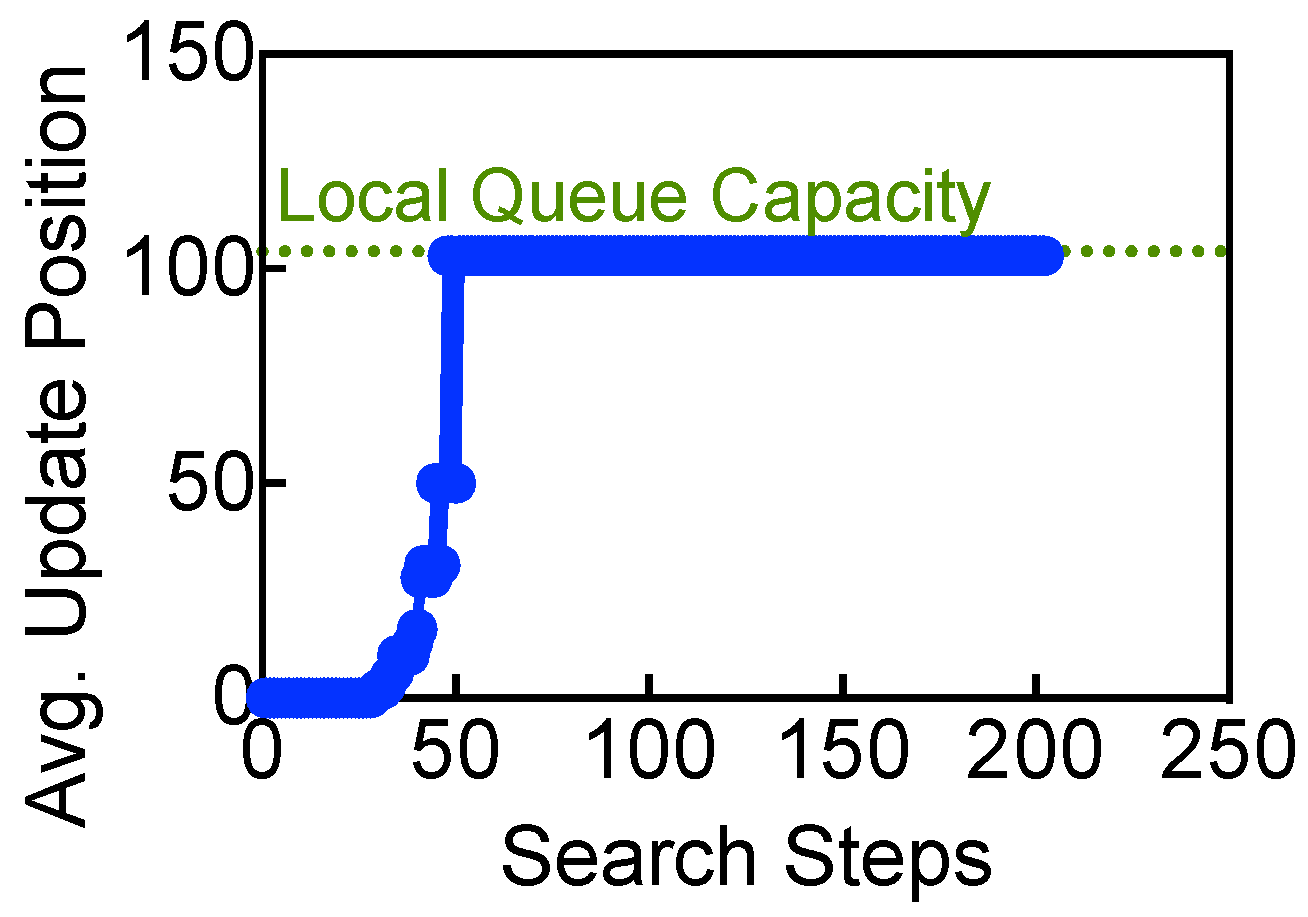
\includegraphics[height=0.98in]{submissions/Minjia2023/figures/insight_PSS_update_position_example}
        \caption{A query's average update positions during searching.
            %\textmd{When $M$ is increasing, \Hammer's search steps are declining while its distance computation is increasing.}
        }
        \label{minjia_fig:insight_PSS_update_position_example}
    \end{minipage}
    %    \caption{\Hammer has much less search steps than \SeqFullName (\SeqShortName) does. The dataset is SIFT1M. They have the same $L=100$. \Hammer has $M=64$.}
    %    \label{minjia_fig:insight_convergence_steps_Top_M_vs_SGS}
\end{figure}




%as when the synchronization frequency is low, the amount of distance computation becomes huge.
%A major reason for slow convergence without any synchronization is that, different worker threads traverse the graph at their own pace; a worker may explore an unpromising area whereas others might already find a promising direction. 
%In this case, the distance computations are statistically inefficient for the worker that is exploring the unpromising area, and it may better help the search process if other threads share their search information with it. 



\noindent\textbf{Synchronization Metrics.}
As shown in Algorithm~\ref{minjia_algo:par_stale_search}, our synchronization frequency is controlled by \texttt{CheckMetrics()}, i.e., it determines when all workers merge their private queues into the global one. 
A possible approach of \texttt{CheckMetrics()} is using exhaustive tuning method to find the proper search steps for global synchronization in terms of the shortest latency and recall guarantee. 
However, this exhaustive method has a couple of disadvantages. 
First, the search procedure for the ideal synchronization point is time-consuming. Given a query, the time complexity of finding the optimal setting of synchronization points is factorial about the total length of the search path.
For a given dataset, this can only be reprocessed offline.
Second, the tuning result is input-sensitive. Even a nuance in datasets or queries may result in total difference synchronization points which need be tuned exhaustively start over. Therefore, although the exhaustive method may provide ideal results, it is impractical.

Here an adaptive \texttt{CheckMetrics()} is proposed based on the update positions of workers. When a worker expands an unchecked candidate, its neighbors are then inserted into the worker's local queue, and \emph{the update position} is defined as the \emph{lowest (best)} position of all newly inserted candidates. Thus, \emph{the average update position} is the mean of all update positions of workers. 
Figure~\ref{minjia_fig:insight_PSS_update_position_example} demonstrates how an example query's average update position changes during the search steps without global synchronization. 
It shows that the average update position increases gradually to the local queue capacity and resides there to the end. 
When the average update position is close to the queue capacity, it indicates that most workers are searching among unpromising area and cannot find good enough candidates to update their local results.
Therefore, the average update position can be used as a metric to determine if all workers need to synchronize their local results to adjust the search order. 

Algorithm~\ref{minjia_algo:check_merge_metric} describes the adaptive \texttt{CheckMetrics()} using the average update position as the metric. Given the queue capacity $L$ and a position ratio $R$, the threshold of the average update position to do synchronizatioin is set as $L\cdot R$. 
If the \emph{checker} find the average update position is greater or equal the threshold (Line~\ref{minjia_algo_line:check_metric}), it returns \texttt{true} indicating a global synchronization in Algorithm~\ref{minjia_algo:par_stale_search}.
Empirically, the ratio $R$ is close to $1.0$, such as $0.9$ or $0.8$. The input vector of all update positions are updated by workers regularly without locks. The return flag is only written by the \emph{checker} who is assigned among workers in a round-robin manner.

%%%%%%%%%%%%%%%%%%
%%% outline
%idea:
%paragraph 1: tuning with exhaustive search cons.: 
%1) input-sensitive
%2) each search takes time 
%cannot do it online.
%explain its complexity; 
%
%paragraph 2: our approach key idea, why it works, why it is interesting.
%
%paragraph 3: explain the algorithm and give an example. 
%%% end outline
%%%%%%%%%%%%%%%%%%

%\iffalse
%A simple approach is to use a static schedule where all threads bulk-synchronize in a fixed step limit, say $I_{sync}$. The hyperparameter $I_{sync}$ can be set through tuning. If it is allowed, the tuning procedure can find a proper value to produce nearly optimal latency performance. However, the downside is that it is hard sometimes to estimate the search space and the tuning might be time-consuming.
%
%Another approach is to use some metrics which are able to reflect the dynamic status of workers so that the synchronization point could be adaptive.
%Figure~\ref{minjia_fig:insight_PSS_sync_frequency_vs_ratio_1st_half} shows how the synchronization frequency influences the \emph{update positions} of workers. During a local search step, a worker updates its private queue by inserting new unchecked candidates. The best (lowest) update position of those new candidates are recorded and an average update position can be produced by using all workers' positions. 
%
%In Figure~\ref{minjia_fig:insight_PSS_sync_frequency_vs_ratio_1st_half}, the ratio value indicates how many average update positions during the whole search is located in the first half of local queues. It shows that when the synchronization frequency is high, the most part of update positions is in the first half of local queues; when the frequency is low, most update positions are in the second half of queues. The results show that the update position is a heuristic metric to reflect workers' status.
%
%Based on this observation, an adaptive \texttt{CheckMetrics()} is provided by using the average update position in Algorithm~\ref{minjia_algo:check_merge_metric}.
%During local search, all workers' best update positions are recorded regularly. The \emph{checker} calculates the average update position and compare it to a threshold. If the position is larger than the threshold, the checker will raise the flag and all workers will then stop local search and conduct a global synchronization. Empirically, the threshold could be set as 80\%-90\% capacity of the queue.
%\fi

Table~\ref{minjia_tab:comp_no_sync_bulk_step} shows preliminary results about the performance comparison between adaptive synchronization and no-synchronization. No-synchronization means each thread performs its local search and only combines the results in the end. The results shows that adaptive synchronization is able to improve search efficiency with fewer distance computation.

\begin{table}[]
    \caption{Comparison between no-sync. and adaptive sync.
        \textmd{8 threads on SIFT1M for Recall@100 0.9. 
            Adaptive sync. check workers' dynamic status and merge queues adaptively.
            \texttt{Lt.} denotes latency. \texttt{Compt.} denotes distance computation.}}
    
    \label{minjia_tab:comp_no_sync_bulk_step}
    \begin{tabular}{|c|c|c|c|c|}
        \hline
        Dataset &               \multicolumn{2}{c|}{no-sync.}               &          \multicolumn{2}{c|}{adaptive sync.}           \\ \cline{2-5}
        &         Lt. (ms.)         &            Compt.            &         Lt. (ms.)         &           Compt.            \\ \hline\hline
        SIFT1M  & \multicolumn{1}{c|}{1.16} & \multicolumn{1}{c|}{125.3 M} & \multicolumn{1}{c|}{0.70} & \multicolumn{1}{c|}{33.1 M} \\ \hline
    \end{tabular}
\end{table}

%\begin{figure}[t]
%    \begin{minipage}[t]{0.23\textwidth}
%        \centering
%        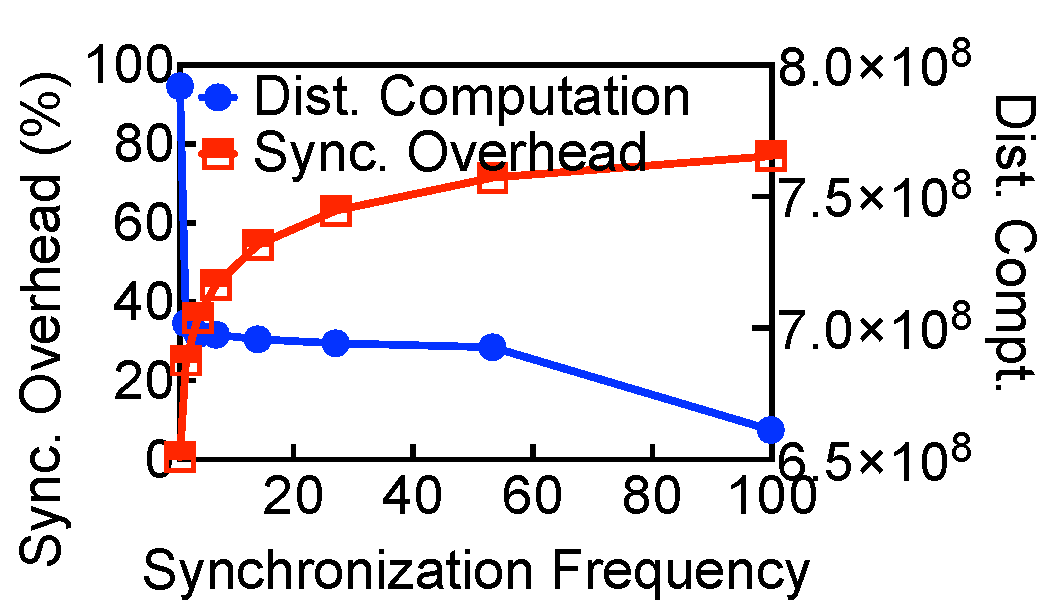
\includegraphics[height=0.98in]{submissions/Minjia2023/figures/insight_PSS_sync_frequency_vs_overhead}
%        \caption{\Hammer's sync. overhead and distance computation vs. sync. frequency.}
%        \label{minjia_fig:insight_PSS_sync_frequency_vs_overhead}
%    \end{minipage}
%    \hfill
%    \begin{minipage}[t]{0.23\textwidth}
%%        \centering
%%        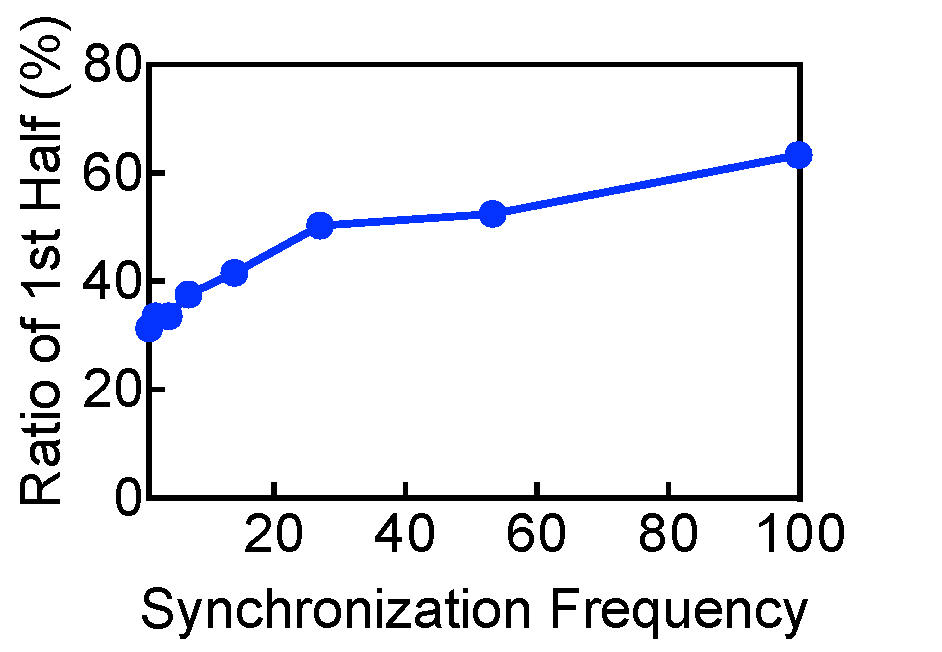
\includegraphics[height=0.98in]{submissions/Minjia2023/figures/insight_PSS_sync_frequency_vs_ratio_1st_half}
%%        \caption{Ratio of the average update position in the 1st half of private queues.
%%            %\textmd{When $M$ is increasing, \Hammer's search steps are declining while its distance computation is increasing.}
%%        }
%%        \label{minjia_fig:insight_PSS_sync_frequency_vs_ratio_1st_half}
%        \centering
%        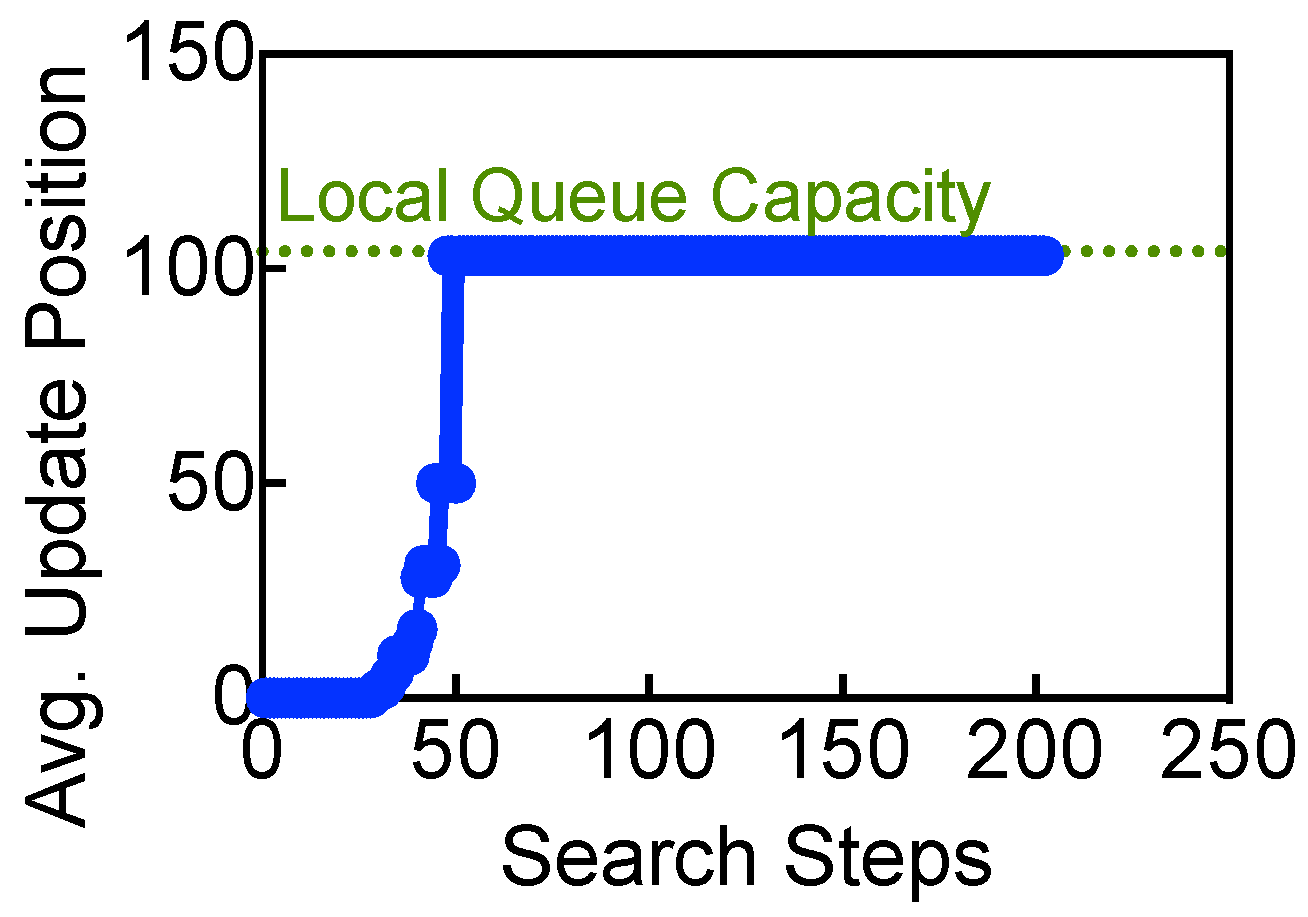
\includegraphics[height=0.98in]{submissions/Minjia2023/figures/insight_PSS_update_position_example}
%        \caption{A query's average update positions during searching.
%            %\textmd{When $M$ is increasing, \Hammer's search steps are declining while its distance computation is increasing.}
%        }
%        \label{minjia_fig:insight_PSS_update_position_example}
%    \end{minipage}
%    %    \caption{\Hammer has much less search steps than \SeqFullName (\SeqShortName) does. The dataset is SIFT1M. They have the same $L=100$. \Hammer has $M=64$.}
%    %    \label{minjia_fig:insight_convergence_steps_Top_M_vs_SGS}
%\end{figure}

\begin{algorithm}[t]
%\small
\DontPrintSemicolon
\caption{CheckMetrics() (by Update Position)}\label{algo:check_merge_metric}
\KwIn{vector of update positions $U$, queue capacity $L$, position ratio $R$, number of workers $T$}
\KwOut{true or false}
$\bar{u} \gets$ average positions of elements in $U$\;
\If{$\bar{u} \geq L \cdot R$} { \label{algo_line:check_metric}
    \Return true\;
}
\Else {
    \Return false\;
}
\end{algorithm}

%%%%%%%%%%%%%
%%% backup
%\begin{algorithm}
%\caption{CheckMetrics() (Update Position Version)}\label{algo:check_merge_metric}
%\begin{algorithmic}[1]
%    \REQUIRE  vector of update positions $U$, queue capacity $L$, position ratio $R$, number of workers $T$
%    \ENSURE true or false
%    \STATE $\bar{u} \gets$ average positions of elements in $U$
%    \IF{$\bar{u} \geq L \cdot R$}
%        \RETURN true
%    \ELSE 
%        \RETURN false
%    \ENDIF
%\end{algorithmic}
%\end{algorithm}
%%% backup
%%%%%%%%%%%%%


%%%%%%%%%%%%%%%%%%%%%%%%%%%%%%%%%%%%%%%%%%%
%%% backup
%\noindent\textbf{Bulk-Step Synchronization with Bounded Order Inversion.} 
%To unleash the full power of multi-core systems, \Hammer performs a unique form of \emph{bounded order inversion} searching so that worker threads do not need to synchronize at every search step in most cases. Specially, \emph{bounded order inversion} means instead of having a strict order through the entire convergence steps, we allow some relaxation of the order as long as the global order becomes consistent again after a given number of steps. 
%This is especially helpful for the multi-path parallel search's performance because global synchronization across multiple threads is still expensive and not very scalable as the number of cores increases. 
%
%\begin{table}[]
%\caption{Comparison between No-sync and Bulk-step Sync
%    \textmd{8 threads on SIFT1M for Recall@100 0.9. 
%            Bulk-step Sync allows workers to share their progress to improve their search efficiency.
%            \texttt{Lt.} denotes latency. \texttt{Compt.} denotes distance computation.}}
%
%\label{minjia_tab:comp_no_sync_bulk_step}
%\begin{tabular}{|c|c|c|c|c|}
%    \hline
%    Dataset & \multicolumn{2}{c|}{No-sync}                            & \multicolumn{2}{c|}{Bulk-step Sync.}                   \\ \cline{2-5} 
%    & Lt. (ms.)            & Compt.                       & Lt. (ms.)            & Compt.                      \\ \hline \hline
%    SIFT1M  & \multicolumn{1}{r|}{1.16} & \multicolumn{1}{r|}{125.3 M} & \multicolumn{1}{r|}{0.70} & \multicolumn{1}{r|}{33.1 M} \\ \hline
%\end{tabular}
%\end{table}
%
%On the other hand, we find that too much order inversion (e.g., no synchronization) could slow down the search convergence -- worker threads spend a lot of time searching non-promising areas, which does not help improve the overall search speed. A major reason for slow convergence without any synchronization is that, different worker threads traverse the graph at their own pace; a worker may explore an unpromising area whereas others might already find a promising direction. In this case, the distance computations are statistically inefficient for the worker that is exploring the unpromising area, and it may better help the search process if other threads share their search information with it. To address it, we introduce bulk-step synchronization with bounded order inversion, which allows worker threads to share their progress periodically and use the latest frontier info in subsequent searches. 
%
%To decide when to perform the bulk-step synchronization, \Hammer supports two mechanisms: the first one is to use a fixed schedule where all threads bulk-synchronize every $I_{sync}$ steps, and $I_{sync}$ is a hyperparameter we set through tuning. We also introduce an ``order-inversion-aware'' approach, where we track the best found local candidate from each worker as a measure of the search quality of each thread. Severe order inversion is detected if the mean of the distances of top candidates is beyond $D\%$ of the smallest distance, and bulk-step synchronization is triggered when a severe order inversion has been detected. In practice, we find that the simple and fixed schedule works pretty well with very minimal hyperparameter tuning cost. We therefore choose the fixed schedule for subsequent experiments.
%{Table~\ref{minjia_tab:comp_no_sync_bulk_step} shows preliminary results about the performance comparison between bulk-step synchronization and no-synchronization. No-synchronization means each thread performs its local search and only combines the results in the end. The results shows that bulk-step synchronization is able to improve search efficiency with fewer distance computation.}
%
%% \minjia{@Zhen, is this what you tried?  I still do not see why this does not work. When D is small, it simply falls back to naive synchronization, and when D is large, it becomes full staleness. There seems to be a sweet spot in between which we can find through experiments. I think it really helps if we have a story here on how to adaptively trigger the bulk-synchronization with staleness awareness.
%%     \zhenfix{Zhen: If I remember correctly, the change of the mean value is not aligned with the merge. The mean value would become fixed far before a merge happens. This is because the top nearest neighbor in a local queue usually can be found in early search steps, which is similar to what happens in the global queue for the \SeqFullName. Given this, the D would either be too small that incurs more merges than necessary, or too large that incurs no merge at all.}}
%%% end backup
%%%%%%%%%%%%%%%%%%%%%%%%%%%%%%%%%%%%%%%%%%%


%%%%%%%%%%%%%%%%%%%%%%%%%%%%%%%%%%%%%%%%%%%
%%% backup
%\subsection{Progressive Multi-Path Search}
%\label{minjia_subsec:progressive_MPS}
%
%%%%% Introduce \ScaleM as an improvement.
%
%To investigate whether multi-path search is needed in the entire search process, we gradually increase the multi-path width (i.e., M) and the number of worker threads every $t$ steps during the search procedure. The intuition is that the search is less likely to get stuck at local minimum in the beginning of the search, so best-first search with single thread can already help the query to get close to near neighbors. As the search moves forward, it becomes more likely that a query will get stuck at local minimum and requires backtracking to escape from local minimum. Therefore, a multi-path search in later phases can better help reduce the convergence steps.  
%
%
%In practice, we find that a simple scaling rule works well. For example, when search begins, we first set a starting value and a maximum value for $M$. The starting value is usually one, and the maximum value can be as large as the number of available hardware threads. Subsequently, every $t$ steps (e.g., $t=1$) we double the value of $M$ until $M$ reaches its maximum. We call this dynamic increase of multi-path search width \ScaleM (\ScaleMShortName). 
%Figure~\ref{minjia_subfig:insight_1T_compt_Scale_M_vs_Top_M_vs_SGS} shows that \ScaleMShortName reduces the amount of redundant significantly in comparison to \Hammer and leads to distance computations close to \SeqShortName. On the other hand, \ScaleMShortName is able to converge as almost fast as \Hammer, as shown in 
%Figure~\ref{minjia_subfig:insight_unchecked_vs_iter_Top_M_Scale_M}. As a result, \ScaleMShortName preserves the fast convergence speeds brought by \Hammer, while with a similar amount of distance computations as \SeqShortName. 
%
%
%\begin{figure}[t]
%    %    \begin{minipage}[t]{0.22\textwidth}
%        \begin{subfigure}[t]{0.23\textwidth}
%            \centering
%            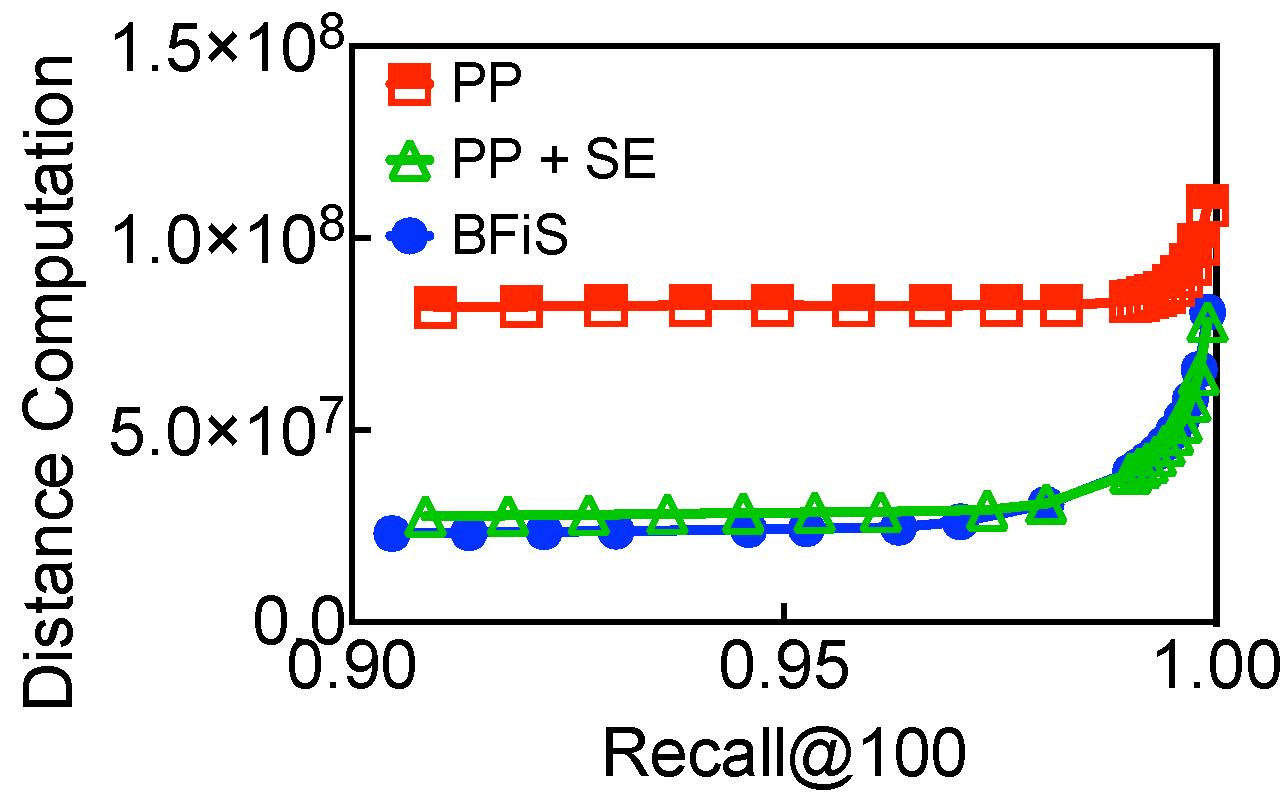
\includegraphics[height=1.1in]{submissions/Minjia2023/figures/insight_1T_compt_Scale_M_vs_Top_M_vs_SGS}
%            \caption{Distance computation of \SeqShortName, \Hammer, and \ScaleMShortName.
%                \textmd{\ScaleMShortName and \SeqShortName have similar distance computations.}}
%            \label{minjia_subfig:insight_1T_compt_Scale_M_vs_Top_M_vs_SGS}
%            %    \end{minipage}
%    \end{subfigure}
%    \hfill
%    %    \begin{minipage}[t]{0.22\textwidth}
%        \begin{subfigure}[t]{0.23\textwidth}
%            \centering
%            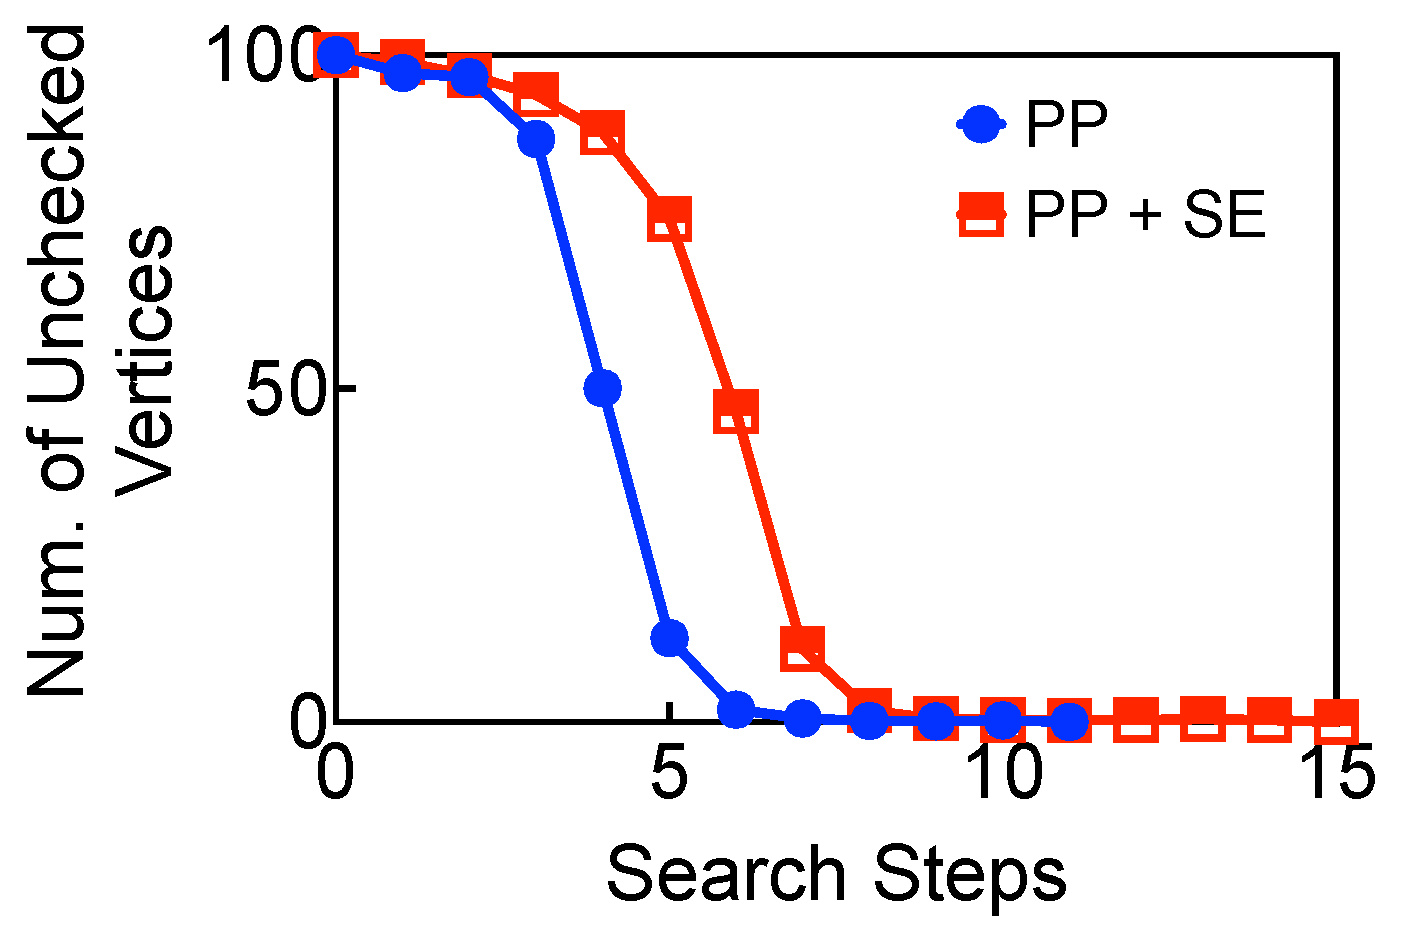
\includegraphics[height=1.05in]{submissions/Minjia2023/figures/insight_unchecked_vs_iter_Top_M_Scale_M}
%            \caption{\#unchecked candidates after each search step. 
%                \textmd{\ScaleMShortName \& \Hammer have similar numbers  of steps.}}
%            \label{minjia_subfig:insight_unchecked_vs_iter_Top_M_Scale_M}
%            %    \end{minipage}
%    \end{subfigure}
%    \caption{Comparison between \Hammer and \ScaleMShortName: distance computation \& search steps.
%        \textmd{$M = 64$.}}
%    \label{minjia_fig:insight_Top_M_vs_Scale_M}
%    \vspace{1em}
%\end{figure}
%%\subsubsection{\FullName Algorithm}
%
%%% end backup
%%%%%%%%%%%%%%%%%%%%%%%%%%%%%%%%%%%%%%%%%%%

%\subsection{Cache Friendly Neighbor Grouping}
%\label{minjia_subsec:neighbor_grouping_reorder}
\subsection{Other Optimizations}

\noindent\textbf{Loosely Synchronized Local Computation.}
There is one potential bottleneck to multi-threaded parallel scaling in Algorithm~\ref{minjia_algo:par_stale_search} on our target architectural platforms (multi-core systems). 
Consider visiting a neighbor of a candidate. This is typically after a check and then an update to a visiting map to ensure that a vertex is calculated once (Line~\ref{minjia_algo_line:stale_check_map}-\ref{minjia_algo_line:stale_update_map}).
In multi-path parallel search, the visiting map is shared by all workers to indicate if a vertex has been visited.
Since multiple threads may access the shared visiting map concurrently, locking or lock-free algorithms are required if we still want to ensure a vertex is visited only once. However, this approach involves significant scalability bottleneck, because it leads to lock contention and sequentialization of updating the visiting map.

We observe that the ANN search algorithm is still correct even if a vertex is calculated multiple times, because the local candidates are guaranteed to be merged back to the global priority queue and the visiting map is also guaranteed to have \emph{eventual consistency} the next time of global synchronization. Furthermore, by inserting memory fences, cache coherence further ensures that the updated visiting map is visible to other cores. Due to the potential out-of-order execution in processors, modern multi-core processors provide \emph{fence} instructions as mechanism to override their default memory access orders. In particular, we issue a fence after a thread updates the visiting map to guarantee a processor has completed the distance computation of the corresponding vertex and has updated the visiting map (otherwise, there is no guarantee the updated visiting map is visible to other cores before next step of global synchronization).

By doing the loosely synchronized local search, we observe that the search algorithm only performs a very small percentage of additional distance computations (less than 5\%) for {SIFT1M} (and similar for other datasets) with 8-way parallelism. This reduces  the overhead from synchronization by 10\% and allows us to avert the issue of non-scaling locking across multi-threading search. This optimization was also considered by Leiserson and Schardl~\cite{benign-race} (termed as "benign races") for their parallel breadth-first search algorithm. 
Furthermore, we use a bitvector to implement the visiting map instead of a byte-array.
% where byte is the minimum data type with Compare-and-Swap (CAS) support. 
This optimization allows the cache to hold the largest possible portion of the visiting map and therefore improves the data locality for memory accesses. 

\noindent{\textbf{Two-Stage Search.}}
In the implementation of \Hammer, the global queue will be filled full of unchecked vertices at first place. Most of those initial vertices are chosen randomly from the graph index, so it is quite common that some of them are far away form the query. Those far away vertices are not promising to be explored and cannot contribute to the final results. If they are assigned to workers immediately, unnecessary distance computation will incur.

To avoid the unnecessary distance computation during the beginning exploration, \Hammer adopts \emph{two-stage search}. The idea is to do one or two expasion of sequential \SeqShortName in the beginning to ``warm up'' the global queue, making its unchecked candidates more promising than initial vertices. This is called the \emph{sequential stage}.
After that, it is followed by the \emph{parallel stage} where all unchecked vertices are assigned to workers for local search. In this way, \Hammer can reduce unnecessary distance computation and also tap into the benefits of parallelization to the greatest extent possible.


\noindent{\textbf{Cache Friendly Neighbor Grouping.}}
When a feature vector is loaded into memory for distance computation, modern CPU architectures actually automatically load vectors from nearby memory locations as well. 
Our neighbor grouping technique taps into this feature to mitigate the two levels of irregularity mentioned in Section~\ref{minjia_sec:overview}.

First, \Hammer \emph{flattens} the graph indices by placing the embeddings of neighbor vertices in consecutive memory, which would avoid one-level of implicit memory addressing and enables a thread to pre-fetch neighbor feature vectors once an active node is selected.  Second, \Hammer also regroups nodes, such that vertices that are likely to be visited during the graph traversal are already pre-load into the CPU memory and cache. Together, these two optimizations increase the cache hit rate and helps speedup the search process. 


One caveat of this approach is that it introduces additional memory consumption, because two neighbor lists may share the same vertex as a common neighbor. It is therefore may require more memory consumption than the original approach.
To avoid increasing the memory consumption, \Hammer takes a hierarchical approach by regrouping only a subset of vertices. In particular, \Hammer divides a graph to a two-level index as shown in Figure~\ref{minjia_fig:fig_reorder}, where only the top-level vertices have their neighbors flattened and stored in consecutive memory, and the bottom-level index stores other vertices using the standard structure. 
In this work, we explore two strategies to graph division: 
     \textbf{Degree-centric}, which puts high in-degree nodes to the top-level of the indices. The intuition is that high in-degree nodes are more frequently accessed, and therefore improving their locality would benefit the most for the overall search efficiency.
     \textbf{Frequency-centric}, which exploits query distribution to figure out which nodes are more frequently accessed and puts those frequently accessed nodes into an optimized index.
Section~\ref{minjia_sec:eval} evaluates both strategies and shows that \Hammer's neighbor grouping strategy brings 10\% performance improvements with selecting only 0.1\% vertices as the top level for a dataset with 100M vertices.



%\begin{figure}[t]
%    \begin{minipage}[t]{0.23\textwidth}
%        \centering
%        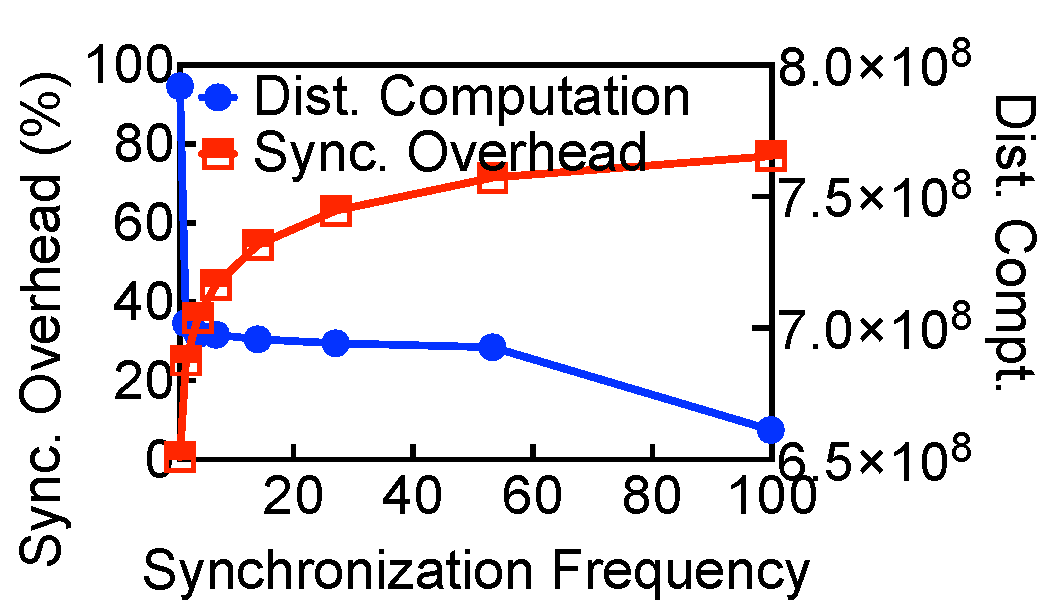
\includegraphics[height=0.98in]{submissions/Minjia2023/figures/insight_PSS_sync_frequency_vs_overhead}
%        \caption{Synchronization overhead and distance computation of \Hammer when synchronization frequency changes.}
%        \label{minjia_fig:insight_PSS_sync_frequency_vs_overhead}
%    \end{minipage}
%    \hfill
%    \begin{minipage}[t]{0.23\textwidth}
%        \centering
%        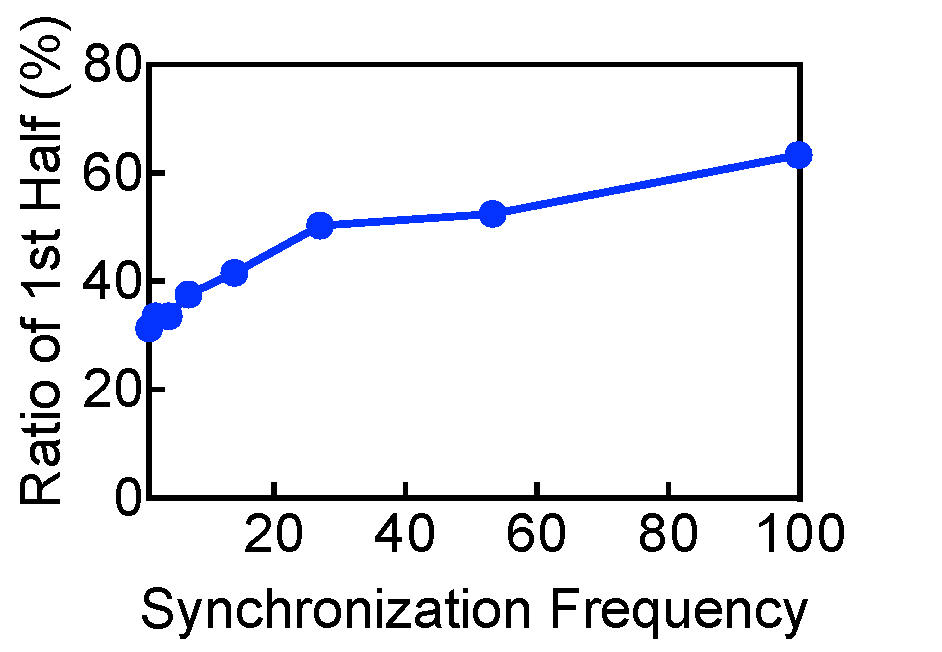
\includegraphics[height=0.98in]{submissions/Minjia2023/figures/insight_PSS_sync_frequency_vs_ratio_1st_half}
%        \caption{Ratio of the average update position in the 1st half of private queues.
%            %\textmd{When $M$ is increasing, \Hammer's search steps are declining while its distance computation is increasing.}
%        }
%        \label{minjia_fig:insight_PSS_sync_frequency_vs_ratio_1st_half}
%    \end{minipage}
%    %    \caption{\Hammer has much less search steps than \SeqFullName (\SeqShortName) does. The dataset is SIFT1M. They have the same $L=100$. \Hammer has $M=64$.}
%    %    \label{minjia_fig:insight_convergence_steps_Top_M_vs_SGS}
%\end{figure}

\begin{figure}
    \centering
    \includegraphics[width=0.45\textwidth]{submissions/Minjia2023/figures/fig_reorder}
    \caption{Example of neighbor grouping and hierarchical data storage. 
            \textmd{
                    Vertices are ranked according to their in-degree. 
                 Vertices are first reordered into new ids according to their ranks.
                    High ranked vertices are stored in an optimized index where every vertex's neighbors' data are stored in consecutive locations right after its own data to make expanding cache-friendly. 
                    Other low ranked vertices are stored in a standard index where the graph index and data vectors are stored separately.}}
    \label{minjia_fig:fig_reorder}
%    \vspace{1em}
\end{figure}

%%%%%%%%%%%%%%%%%%%%%%%%%%%%%%%%%%%%%%%%%%%
%%% backup
%\subsection{Tuning and Adaptation}
%
%As a fixed configuration for a dataset and hardware architecture is not always the best solution, the configuration of \Hammer needs to be tuned case by case in an efficient manner. 
%There are two important parameters that control \Hammer's performance: $L$ and $I_{sync}$.
%{
%$L$ is the length of the priority queue, for both the global one and local ones.
%$I_{sync}$ is the synchronization intervals for bulk-synchronization.
%}
%$L$ is able to influence the recall of final results. 
%When $L$ increases, more vertices are visited during the search, so that the recall will be improved.
%$I_{sync}$ controls how many vertices will be expanded before merging. 
%If $I_{sync}$ is too small, some local candidates might be left unchecked, and the merging frequency will be too high.
%If $I_{sync}$ is too large, even though all local candidates will be expanded, some of them are inevitably dropped after merging, causing the distance computation increasing.
%Since both the search space of $L$ (e.g., 100-200 with an interval of 10) and $I_{sync}$ (e.g., 10--100) are small, \Hammer can find the optimal execution configuration with just a few hundred calibration runs. This calibration process is often called once offline, and then the optimized search algorithm is repeatedly used for processing upcoming query requests.
%
%
%% How to choose L and X?
%We further find a heuristic to decide $L$ and $I_{sync}$ that works well in practice that largely avoids the calibration phase. 
%Assume a given recall of $K$ nearest neighbors,
%and assume $L_0$ is the value of $L$ for \SeqFullName to achieve the given recall. 
%For \FullName with $T$ workers, $L$ can be set as $L = L_0 / T$ as long as $L_0 / T \ge K$, 
%and $I_{sync}$ can be set as $X = L_0 / T$ as long as $L_0 / T > 1$. More details are shown in Algorithm~\ref{minjia_algo:get_L_for_PSS} and ~\ref{minjia_algo:get_X_for_PSS}.
%This way ensures to fully use all local queues and to limit the synchronization overhead.
%Please note that $L$ cannot be too small with respect of $K$, otherwise we may never meet the required recall.
%
%\begin{figure}
%    \centering
%    \includegraphics[width=0.45\textwidth]{submissions/Minjia2023/figures/fig_reorder}
%    \caption{Example of neighbor grouping and hierarchical data storage. 
%        \textmd{
%            Vertices are ranked according to their in-degree. 
%         Vertices are first reordered into new ids according to their ranks.
%            High ranked vertices are stored in an optimized index where every vertex's neighbors' data are stored in consecutive locations right after its own data to make expanding cache-friendly. 
%            Other low ranked vertices are stored in a standard index where the graph index and data vectors are stored separately.}}
%    \label{minjia_fig:fig_reorder}
%    \vspace{1em}
%\end{figure}
%
%%Algorithm~\ref{minjia_algo:get_L_for_PSS} shows how to determine the value of $L$.
%\begin{algorithm}
\caption{Compute $L$ for \FullName}\label{algo:get_L_for_PSS}
\begin{algorithmic}[1]
\REQUIRE value of $K$, queue capacity $L_0$ of \SeqShortName, $T$ workers 
\ENSURE value of $L$ for \FullName
\IF{$L_0 < K$}
    \RETURN $L_0$
\ELSIF{$(L_0 / T) < K$)}
    \RETURN K
\ELSE
    \RETURN $L_0 / T$
\ENDIF
\end{algorithmic}
\end{algorithm}
%
%%Algorithm~\ref{minjia_algo:get_X_for_PSS} shows how to determine the value of $I_{sync}$.
%\begin{algorithm}
\caption{Compute $I_{sync}$ for \FullName}\label{algo:get_X_for_PSS}
\begin{algorithmic}[1]
\REQUIRE queue capacity $L_0$ of \SeqShortName, $T$ workers 
\ENSURE value of $I_{sync}$ for \FullName
\IF{$L_0 / T < 1$}
    \RETURN $1$
\ELSE
    \RETURN $L_0 / T$
\ENDIF
\end{algorithmic}
\end{algorithm}
%%% end backup
%%%%%%%%%%%%%%%%%%%%%%%%%%%%%%%%%%%%%%%%%%%

